%NOTE
\documentclass{article}
\usepackage[margin=1.0in]{geometry}
\usepackage{titling}
\usepackage{graphicx}
\usepackage{float}
\usepackage[T1]{fontenc}

\begin{document}
	
	%%% title
	\setlength{\droptitle}{-5em}
	\title{Journal}
	\date{}
	\author{}
	\maketitle
	
	%%% first section
	\section{Review}
	\section*{Inequalities}
	\textbf{One-Variable Inequalities}\\ 
	In the case of an inequality like  $-3 \leq 1-2x < 4x$ \\
	You can split it up into two equations:  $-3 \leq 1-2x$, $1-2x < 4x$\\
	As both are true, this is an "and" statement: 
	$-3 \leq 1-2x$ and $1-2x < 4x$ \\
	From here, you can simplify to get a final answer: 
	$2x \leq 4$ $\rightarrow$ $x \leq 2$ and $-6x < -1$ $\rightarrow$ $x > 1/6$ \\
	Finally: 
	$x \leq 2$ AND $x > 1/6$\\
	Alternatively: $1/6 < x \leq 2$ \\\\
	\textbf{Two-Variable Inequalities}\\ 
	With a two-variable inequality like $y > -x^3 +4$ \\\\
	1) First graph it: \\
	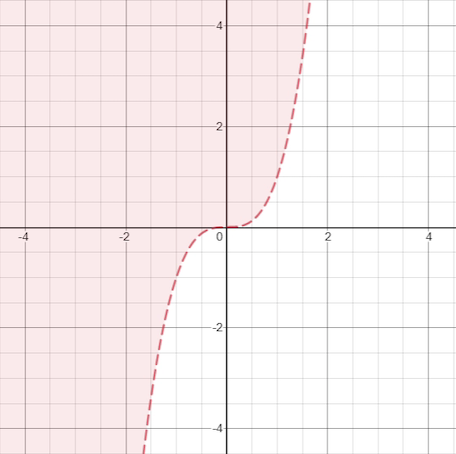
\includegraphics[scale=0.30]{pics/j92v1}
	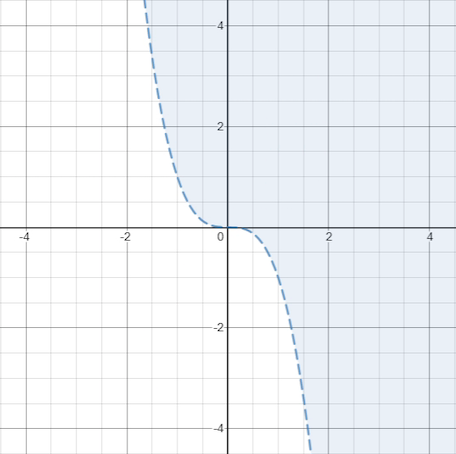
\includegraphics[scale=0.30]{pics/j92v2}  
	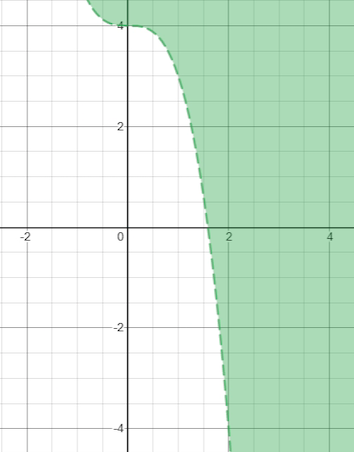
\includegraphics[scale=0.30]{pics/j92v3} \\
	In this case, I am graphing the base function, $y=x^3$ \\
	Then flipping it across the y-axis: $y=-x^3$ \\
	Finally adding the +4 and transforming up 4: $y=-x^3+4$ \\ \\
	2) Second, test a point $(0, 0)$: \\
	We find that it is out of the solution set. \\
	This means that the area this inequality represents is above the line. \\
	We know it is dotted as $>$ or $<$ inequalities are non-inclusive. \\\\
	\textbf{Absolute Value Inequalities} \\
	Although they share similarities to normal inequalities, they are solved differently. 
	\\\\ In the case of $3|2x+1|>12$:\\ \\
	1) Isolate the absolute value: 
	$|2x+1|>4$  \\ \\
	2) Separate into 2 equations. Absolute value inequalities are or, not and. \\
	\\Equation 1: $+(2x+1) > 4$ $\rightarrow$ $2x > 3$ $\rightarrow$ $x>2/3$
	\\Equation 2: $-(2x+1) > 4$ $\rightarrow$ $2x+1< -4$ $\rightarrow$ $2x < -5$ $\rightarrow$ $x < -5/2$ \\ \\
	Finally: $x < -5/2$ OR $x>2/3$ \\
	\section*{Quadratic Forms}
	\textbf{General Form}: $ax^2 + bx + c$ \\
	Example: $x^2 + 6x + 9$ \\
	\textbf{$A$} determines whether the parabola opens up/down (-a is down)\\
	\textbf{$B$} moves the axis of symmetry from side to side\\
	\textbf{$C$} is the Y intercept\\ 
	\textbf{Vertex:} ($-b/2a$), ($f(-b/2a)$) (Ex: $(-3)$, $(0)$) \\
	\textbf{Axis of Symmetry:} $-b/2a$ (Ex: $-3$)\\
	\textbf{Y-Intercept:} $C$ (Ex: 9)\\
	\textbf{X-Intercept:} Solve (Ex: -3)\\ \\
	\textbf{Vertex Form}: $a(x-h)^2+k$ \\
	Example: $-2(x-4)^{2}+2$\\
	$(-H, K)$ is the vertex, $A$ is the same as general form \\ 
	\textbf{Vertex:} ($-h, k$) (Ex: $(4, 2)$)\\
	\textbf{Axis of Symmetry:} $h$ (Ex: $4$)\\
	\textbf{Y-Intercept:} Set $x=0$, solve for $y$ (Ex: -30) \\
	\textbf{X-Intercept:} Set $y=0$, solve for $x$ (Ex: (3, 0), (5, 0))\\ \\
	\textbf{Factored Form}: $a(x-r)(x-s)$ \\
	Example: $(x+3)(x+2)$ \\
	$(-R, -S)$ are the X intercepts, A is the same as general form \\ 
	\textbf{Vertex:} Get the average of the $x$-intercepts, substitute (Ex: (-2.5, -0.25))\\
	\textbf{Axis of Symmetry:} $(r+s)/2$ (Ex: -2.5)\\
	\textbf{Y-intercept:} Set $x=0$, solve for $y$ (Ex: 6)\\
	\textbf{X-Intercept:} $(-r, -s)$ (Ex: (0, -3), (0, -2)) 
	\section*{Quadratic Patterns}
	\textbf{Difference of Squares} \\
	$a^2 - b^2 = (a-b)(a+b)$ \\
	Example: $9x^2 -64 = (3x + 8 )(3x-8)$ \\ \\
	\textbf{Difference of Cubes}\newline
	$a^3 + b^3 = (a+b)(a^2 - ab +b^2)$\\
	(On the right side, first sign is same, second is opposite, last is +). \\
	Example: $2^3 + 5^3 = (2 + 5)(2^2 - 10 + 5^2)$ \\
	\\
	\textbf{Perfect Square Trinomial} \\
	Must satisfy requirement of $b^2=4ac$ \\
	Example: $x^2+6x+9$ \\
	$6^2 = 4*1*9$ $\rightarrow$ $36=36$ \\
	$(x+3)(x+3)$ 
	\section*{Quadratic Methods}
	\textbf{Factor By Grouping} \\
	$3t^3 + 6t^2 + 2t + 4$  \\
	Take out common monomials for first 2 and last 2 (can rearrange nums) \\
	$3t^2(t + 2) + 2(t+2)$ \\
	$(3t^2 + 2) (t+2)$ \\ \\
	\textbf{Into 2 Binomials} \\
	$x^2 + 7x + 12$ \\
	Fill in last number of each paren: $( + 4) ( + 3)$ - have to add to 7, multiply to 12 \\
	$x^2 + bx + c$ \\
	(  +d) (  +e) - D and E have to add up to B and multiply to C \\\\
	\textbf{Quadratic Formula} : $x=\frac{-b\pm\sqrt{b^2-4ac}}{2a}$ \\
	Example: $x^2+3x+2$ \\
	$x=\frac{-3\pm\sqrt{3^2-4*1*2}}{2*1}$ \\
	$x=\frac{-3\pm\sqrt{1}}{2}$ \\
	Finally: $-1$ and $-2$ are returned from the formula. \\ \\
	\textbf{Completing the Square} \\
	Example: $x^2+4x+1$ \\
	1) Divide equation by $a$ \\
	Ex: Skip, $a=1$\\
	2) Move $c$ to the opposite side of the equation \\
		Ex: $x^2+4x = -1$ \\
	3) Create a perfect square trinomial by completing operations on each side \\
		Ex: $x^2 + 4x + 4 = 3$\\
	$(x+2)^2 = \pm 3$\\
	$\rightarrow$ Resulting equation should follow the form $(x + p)^2 = \pm q$\\
	4) $\sqrt{}$ equation \\
		Ex: $x+2 = \pm ~1.73$ \\
	5) Solve for x\\
		Ex: $x = ~-3.73$ or $x = ~-0.27$
	
	\section{Question}
	I am curious as to whether there is a shortcut to completing the square like how the quadratic formula is.
	
	\section{Notes to Ms. Zanca}
	I tried typing my journal up this time because it was a bit longer. Hopefully it's fine. The quadratic patterns, methods, forms all took quite a bit of space and I also hope it's not too long to read. On another note, I had a nice, relaxing, weekend and am ready to return to school. I've also been practicing on IXL a bit, albeit inconsistently. I'm trying to work it into my schedule right now, but I'm just getting busier and busier.
	
\end{document} 
